\documentclass[20pt,landscape]{foils}
\usepackage{amsmath, amssymb, amsthm}
\usepackage{amstext}
\usepackage{amsgen}
\usepackage{amsxtra}
\usepackage{amsgen}
\usepackage{amsthm}
\usepackage{color}
\usepackage{hyperref}
%\usepackage{pause}
\usepackage{graphicx}
\usepackage{epsfig}
%\usepackage{geometry}
%\geometry{headsep=3ex,hscale=0.9}
\newcommand{\bd}{\textbf}
\newcommand{\no}{\noindent}
\newcommand{\un}{\underline}
\newcommand{\bi}{\begin{itemize}}
\newcommand{\ei}{\end{itemize}}
\newcommand{\be}{\begin{enumerate}}
\newcommand{\ee}{\end{enumerate}}
\newcommand{\bc}{\begin{center}}
\newcommand{\ec}{\end{center}}
\newcommand \h {\hspace*{.3in}}
\newcommand{\bul}{\hspace*{.3in}{\textcolor{red}{$\bullet$ \ }}}
\newcommand{\xbar}{\bar{x}}
\rightheader{Stat 330 (Fall 2015): slide set 14}

\begin{document}
\LogoOff

\foilhead[1.3in]{}
\centerline{\LARGE \textcolor{blue}{Slide set 14}}
\vspace{0.3in}
\centerline{\large Stat 330 (Fall 2015)}
\vspace{0.2in}
\centerline{\tiny Last update: \today}
\setcounter{page}{0}

\foilhead[-.75in]{\textcolor{blue}{Gamma Example (Baron 4.7)}}
\no {\textcolor{magenta}{Compilation of a computer program consists of 3 blocks that are processed sequentially, one after the other.
Each block takes Exponential time with mean  of 5 minutes, independently of other blocks.}}\\[.1in]
{\textcolor{cyan}{(a) Compute the expectation and variance of the total compilation time.}}\\[.2in]
For a Gamma random variable T with $\alpha=3$ and $\lambda=1/5$,
\bc
 $E(T)=\frac{3}{1/5}=15$ (min) and $Var(T)=\frac{3}{(1/5)^2}= 75$ (min)
\ec
{\textcolor{cyan}{(b) Compute the probability for the entire program to be compiled in less than 12 minutes. }}\\[.2in]
This can be done using repeated integration by parts (see Baron p.87). \\[.1in]

\foilhead[-.75in]{\textcolor{blue}{Gamma Example (Cont'd)}}
\no However we will use the \emph{Gamma-Poisson} formula:\\[.1in]
{\textcolor{magenta}{For  $T \sim Gam(\alpha,\lambda)$}} and {\textcolor{magenta}{$X \sim Po(\lambda t)$,}} 
$${\textcolor{cyan}{P(T>t)=P(X<\alpha) \text{\ and \ } P(T \le t)=P(X \ge \alpha)}}$$
Need $P(T<12)$ where $T \sim Gam(3,1/5)$. \\[.1in]
Note that $t=12$ so $X \sim Po(12/5)$ i.e., $X \sim Po(2.4)$. \\[.1in]
From the Gamma-Poisson formula,
\bc
 $P(T<12)=P(T \le 12)=P(X \ge 3)=1- Po_{2.4}(2)=1-0.5697$
\ec

\foilhead[-.75in]{\textcolor{blue}{Erlang distribution}}
\no {\textcolor{magenta}{Hits on a web page}} {\textcolor{cyan}{Recall: we modeled waiting times until the first hit as $Exp(2)$. How long do we have to wait for the second hit?}}\\[.1in]
\no  To calculate waiting time for the second hit, we add 
    the waiting times until the first hit and the time between the 
    first and the second hit.\\[.1in]
\no  Let  $Y_{1}$=the waiting time until the first hit. Then $Y_{1} \sim $ Exponential with $\lambda=2$\\[.1in]
\no Let $Y_{2}$, the time between first and second hit.  By the memoryless property of the exponential 
    distribution, $Y_{2}$ has the same distribution as waiting time for the first hit. \\[.1in]
\no That is $Y_{2} \sim $ Exponential with $\lambda=2$\\[.1in]
\no  We want the total time for the second hit $X := Y_{1} + Y_{2}$.\\[.1in]
\no This is the sum of two independent exponential random variables.

\foilhead[-.75in]{\textcolor{blue}{Erlang distribution (cont'd)}} 
\no If $Y_{1}, \ldots, Y_{k}$ are $k$ independent exponential random 
    variables with parameter $\lambda$, their sum $X$ has an  {\textcolor{magenta}{ Erlang 
    distribution}}:
    $$X := \sum_{i=1}^{k} Y_{i}$$
    \no $\text{ is Erlang}_{(k, \lambda)}$. The {\it Erlang density} $f_{k,\lambda}$ is 
    $$f(x) =\frac{\lambda^k}{(k-1)!} x^{k-1} e^{-\lambda x}\qquad	\text{ for } x \ge 0 $$
 \no where   $k$ is called the  {\textcolor{magenta}{stage parameter}}, $\lambda$ is the  {\textcolor{magenta}{
    rate parameter}}.\\[.2in]
 \no Note this is the same density as that of $Gamma(k,\lambda)$   with $\alpha=k$ is an integer.
\foilhead[-.75in]{\textcolor{blue}{Erlang distribution (cont'd)}} 

\no {\textcolor{magenta}{Expected value}} and {\textcolor{magenta}{variance}} of an Erlang distributed 
variable $X$ can be computed using the properties of expected value and variance for  sums 
of independent random variables:
\begin{eqnarray*}
    E[X] &=& E[\sum_{i=1}^{k} Y_{i}] = \sum_{i=1}^{k} E[Y_{i}] = k 
    \cdot \frac{1}{\lambda} \\
    Var[X] &=& Var[\sum_{i=1}^{k} Y_{i}] = \sum_{i=1}^{k} Var[Y_{i}] = 
    k
    \cdot \frac{1}{\lambda^{2}} \\
\end{eqnarray*}
\no Alternatively, we can use the formulas for the {\textcolor{magenta}{expectation and variance  of $Gamma (k,\lambda)$ random variable}}.\\[.1in]
\no This so because {\textcolor{cyan}{$Erlang(k,\lambda)$ distribution is the same as a $ Gamma(k,\lambda)$ distribution where $k$ is an integer.}
\foilhead[-.75in]{\textcolor{blue}{Erlang distribution (cont'd)}} 
\no Thus, in order to compute the distribution function, we  can use the Gamma-Poisson formula.\\[.1in] 
\no We need the cdf of the Erlang random variable $X$ denoted by $\text{Erlang}_{k,\lambda}(x)$\\[.1in]
$$\text{Erlang}_{k,\lambda}(t)= P( X \le t)$$ 

\no In order to use the Gamma-Poisson formula, we now consider distribution of $X$ as $X \sim Gamma(k,\lambda$)\\[.1in]
\no From  Gamma-Poisson formula, $$P(X \le t)=P(Y \ge k) \text{ where } Y \sim Po(\lambda t )$$  
\no Thus $$\text{Erlang}_{k,\lambda}(t)=   P(Y \ge k)=1- P(Y \le k-1)= 1-Po_{\lambda t} (k-1)   $$ 
 
 
 
\foilhead[-.8in]{\textcolor{blue}{Erlang distribution: Example}}\vspace*{1mm}
\no {\textcolor{magenta}{Hits on a web page (continued)}}\\[.1in]
\no 1. {\textcolor{cyan}{ What is the density of the waiting time until the second hit?}}\\[.1in]
\no We previously defined $X$ , as the sum of two 
exponential variables, each with rate $\lambda = 2$.\\[.1in]
\no Thus $X$ has an Erlang distribution with stage parameter 2; thus, the density of $X$ is\\[.1in]
\hspace*{1in}$f_{X}(x) = f_{k, \lambda}(x) = 4 x e^{-2 x} \qquad	\text{ for } x \ge 0$\\[.15in]
\no 2.  {\textcolor{cyan}{Find the probability that we have to wait $>$ 1 min for the $3^{rd}$ hit.}}\\[.1in]
\no $Z$ := waiting time until the third hit has an Erlang$_{(3, 2)}$ distribution. Thus\\[.1in]
$ P( Z > 1) = 1 - \text{Erlang}_{3,2}(1) = 1 - (1 - Po_{2 \cdot 1}(3 -1)) = 
    Po_{2}(2) = 0.677$\\[.15in]
\no {\textcolor{cyan}{We will come across the Erlang distribution again, when modelling the 
waiting times in queueing systems, where customers arrive with a 
Poisson rate and need exponential time to be served.}}   

\foilhead[-.8in]{\textcolor{blue}{Normal distribution}}\vspace*{2mm}
\no {\textcolor{magenta}{The {\it normal density} is a ``bell-shaped'' density. The density has two parameters: $\mu$ and $\sigma^{2}$ and is}} 
\[
f_{\mu, \sigma^{2}}(x) = \frac{1}{\sqrt{2 \pi \sigma^{2}}} 
e^{-\frac{(x-\mu)^{2}}{2 \sigma^{2}}} \qquad \text{ for } -\infty<x<\infty
\]
\no The expected value and variance of a normal distributed r.v. $X$ are:
\begin{eqnarray*}
    E[X] &=& \int_{-\infty}^{\infty} x f_{\mu. \sigma^{2}}(x) dx = 
    \ldots = \underline{\mu} \\
    Var[X] &=& \int_{-\infty}^{\infty} (x - \mu)^{2} f_{\mu. \sigma^{2}}(x) dx = 
    \ldots = \underline{\sigma^{2}}. \\
\end{eqnarray*}
\no Thus, the parameters $\mu$ and $\sigma^{2}$ are actually the mean and the
variance of the $N(\mu,\sigma^2)$ distribution.
\foilhead[-.5in]{\textcolor{blue}{Normal densities for several 
    parameters}}\vspace*{.1in}
    
\centerline{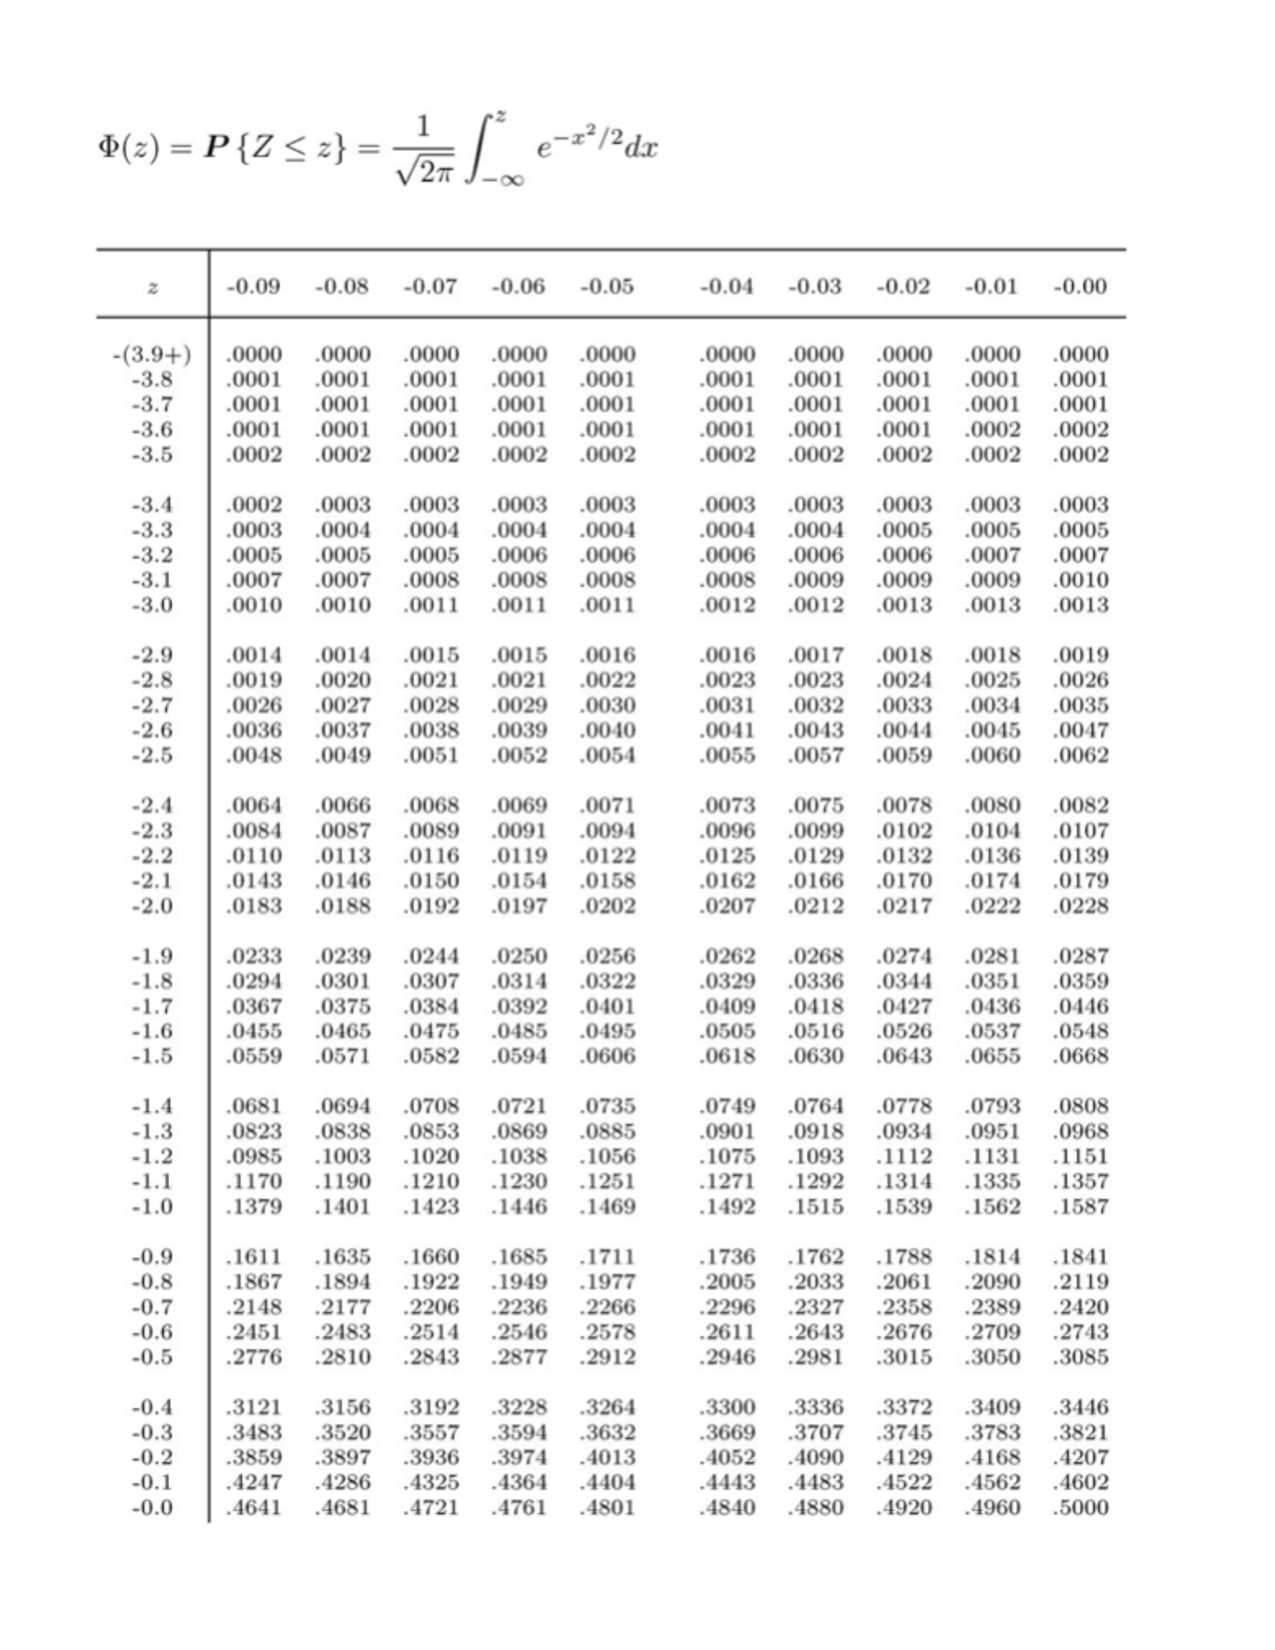
\includegraphics[scale=.8]{normal.pdf}}   
\no {\textcolor{magenta}{$\mu$ determines the location of the peak on the 
    $x-$axis, $\sigma^{2}$ determines the ``width'' of the bell.}} 
    
\foilhead[-.8in]{\textcolor{blue}{Normal distribution (cont'd)}}\vspace*{2mm}    
\no  {\textcolor{magenta}{The cumulative distribution function (cdf) of $X$ is}}\\[.1in]
\hspace*{1in}$N_{\mu, \sigma^{2}}(t)  := F_{\mu, \sigma^{2}}(t)  = \int_{-\infty}^{t} 
f_{\mu, \sigma^{2}}(x) dx$\\[.15in]
\no  Unfortunately, there does not exist a closed form for this 
integral. However, to get probabilities means we need to 
evaluate this integral. \\[.15in] 
\no Fortunately, tables of the cdf of  {\textcolor{magenta}{standard normal distribution $N(0,1)$,the normal distribution that has mean 0 and a variance of 1}}, are available.\\[.16in]
\no  {\textcolor{magenta}{We can use these tables to compute the cdf of the normal distribution $N(\mu,\sigma^2)$ for any set of values of $\mu$ and $\sigma$. How?}}\\[.1in]
\no We use the fact that $X \sim N(\mu,\sigma^2)$ can be standardized to obtain a $Z$ random variable $Z \sim N(0,1)$ as follows:
 $$Z =\frac{X - \mu}{\sigma}$$
 
\foilhead[-.8in]{\textcolor{blue}{Standard Normal distribution }}\vspace*{2mm} 
\no IF $X \sim N(\mu, \sigma^{2})$ then $ Z= \frac{X - \mu}{\sigma} \sim N(0,1)$.\\[.1in]
no Thus\\[.15in]
\no \hspace*{2in} $E[Z] = \frac{1}{\sigma} (E[X] - \mu) = 0$ \\[.1in]
\no \hspace*{2in} $	Var[Z] = \frac{1}{\sigma^{2}} Var[X] = 1$\\[.15in]
\no It is common practice to denote the cdf $N_{0, 1}(t)$ by $\Phi(t)$ (more commonly represented as $\Phi(z)$) \\[.1in]
\no The values of the $\Phi(z)$  are tabulated in tables usually called stanadard normal tables (or Z tables); however, these tables are (sometimes) only available for positive values of z\\[.1in]
\no This table is sufficient because, $\Phi(-z) = 1 - \Phi(z)$ as $f_{0,1}$ is symmetric around 0.
    
\foilhead[-.8in]{\textcolor{blue}{Standard Normal distribution (cont'd) }}\vspace*{8mm}     
           
       \centerline{\includegraphics[scale=.8]{normal2.pdf}}
\no Recall,  the area to the left of the graph up to a specified vertical line  at $z$ represents 
    the probability  $P(Z<z)$\\[.1in]
\no It's easy to see, that the area in the lkeft tail is equal to the area in the right tail:  
$$P(Z \le -z) = P(Z \ge +z).$$
\no This is true because $P(Z \ge  +z) = 1 - P(Z \le z)$, which proves the above statement.

\foilhead[-.8in]{\textcolor{blue}{Using the Z-table }}\vspace*{5mm}
\no Suppose $Z$ is a standard normal random variable. 
\begin{enumerate}
	\item[\bul]  $P(Z < 1) = \Phi(1) \stackrel{\text{straight look-up}}{=} 0.8413.$	
	\item[\bul]  $P(0 < Z < 1) = P(Z < 1) - P (Z < 0) = \Phi(1) - \Phi(0)  
	\stackrel{\text{look-up}}{=} 0.8413 - 0.5 = 0.3413.$
	\item[\bul] $P(Z < -2.31) = 1 - \Phi(2.31) \stackrel{\text{look-up}}{=} 1 - 
	0.9896 = 0.0104.$\\
  or $P(Z<-2.31) = \Phi(-2.31) = 0.0104$.
	\item[\bul]
    $P(|Z| > 2) = P(Z < -2) + P(Z > 2) = 2 ( 1- \Phi(2)) \stackrel{\text{look-up}}{=} 
	2 (1 - 0.9772) = 0.0456.$\\
    or $P(|Z| > 2) = P(Z < -2) + P(Z > 2) = 2 \Phi(-2) \stackrel{\text{look-up}}{=} 
	2 \times 0.0228 = 0.0456.$
    \end{enumerate}
\foilhead[-.8in]{\textcolor{blue}{Using the Z-table (cont'd) }}\vspace*{8mm}
\no Suppose, $X \sim N(1,2)$ and that we need to calculate $P( 1 < X < 2) $\\[.15in]
    {\it
    A standardization of $X$ gives $Z := \frac{X-1}{\sqrt{2}}$. Thus:
    \begin{eqnarray*}
	P(1 < X < 2) &=& P\left( \frac{1 -1}{\sqrt{2}} < \frac{X-1}{\sqrt{2}} < 	\frac{2 - 1}{\sqrt{2}}\right)= \\
	&=& P ( 0 < Z < 0.5 \sqrt{2}) = \Phi(0.71) - \Phi(0) \\[.1in]
	&=& 0.7611 - 0.5 = 0.2611.
    \end{eqnarray*}
    }
\no Note that the standard normal table only shows probabilities for $z < 
3.99$. This is all we need, though, since $P( Z \ge 4) \le 0.0001$.\\[.15in]
\no {\textcolor{magenta}{Review Examples 4.10, 4.11, and 4.12 from Baron}
\end{document}   





  









